\section*{Problem No.3} \label{sec:prob3}
Given the PDE along with boundary conditions 
\[
\epsilon u_{xx}-exp(-|u|)u+g =0,\\
u(0)=u(1)=0
\]
We can approximate the second derivative using the 3-point second-order discritzation 
\[
u_{xx}(x_{j}) \approx \frac{u_{j-1}-2u_{j}+u_{j+1}}{\Delta x^{2}}
\]
where $x_{j}=j\Delta x$ for $j=0 \cdots N+1$ and $\Delta x = \frac{1}{N+1}$ and thus $u_{j}\approx u(x_{j})$. The PDE then becomes 
\[
\frac{\epsilon}{\Delta x^{2}} \left(u_{j-1}-2u_{j}+u_{j+1}\right) - exp(-|u_{j}|)u_{j}+g=0
\]
When the problem is descrtized on $N$ mesh points, we will get $N-2$ in $N$  unknowns and the two boundary conditions will provide the additional two equations. The system of equations is nonlinear and Newton's method can be used to solved it by re-formulating the problem as solve for the roots of the following equation
\[
A(\overrightarrow{u}) + F(\overrightarrow{u})=0
\]
where $F(\overrightarrow{u}) = -exp(-|u_{j})u_{j}+g$ and 
\[
A = \frac{\epsilon}{\Delta x^{2}}
\left( 
\begin{array}{cc cc cc}
-2 & 1 &    &   &   & \\
1 & -2 & 1  &   &   & \\
  & \ddots & \ddots   & \ddots    &   & \\
  & & \ddots & \ddots   & \ddots   & \\
  &   &   & 1  & -2 &1 \\
  &   &   &    & 1 &-2 \\
\end{array} 
\right)
\]

In order to use Newton method, we estimated the Jacobian using finite difference. We note that the Jacobian is tridiagonal matrix and the code from \cite{doi:10.1137/1.9780898718898} is used in order to estimate the banded Jacobian efficiently where a column only needs three new function evaluations. 
\paragraph{Initial Guesses:} The first initial guess taken by considering $u$ and $u_{xx}$ are small and taking the limit $\epsilon =0$. Thus, the initial guess in that case is $u_{j}=g$ for $ j=2 \cdots N-1$ where $N$ is the total number of mesh points. The second initial guess is taken by considering $u$ is large and thus $exp(-|u|)$ is small. From that, we get the initial guess as $u_{j}=-\frac{1}{2}\frac{g}{\epsilon}x^{2}$.

Solving for these two initial guesses gave the solution as shown in Figure \ref{fig:prob3} left and middle for the first and second initial guess respectively. 

The third initial guess was found by taking weighted sum of the first two such that 
$u_{i3} = \alpha u_{i1} + (1-\alpha u_{i2})$ where $u_{i3}$ is the third initial guess we are looking for using the first initial guess $u_{i1}$ and second one $u_{i2}$ by doing binary search to find the right value of $\alpha$. Each iteration in the binary search would measure 2-norm of the obtain solution and update either the upper or lower bound of $\alpha$ (which are set initially to 1 and 0). The third solution was found with $\alpha = 0.999999098479748$ and shown in Figure \ref{fig:prob3} (right). 
 

\begin{figure}[H]
 \centering  
   {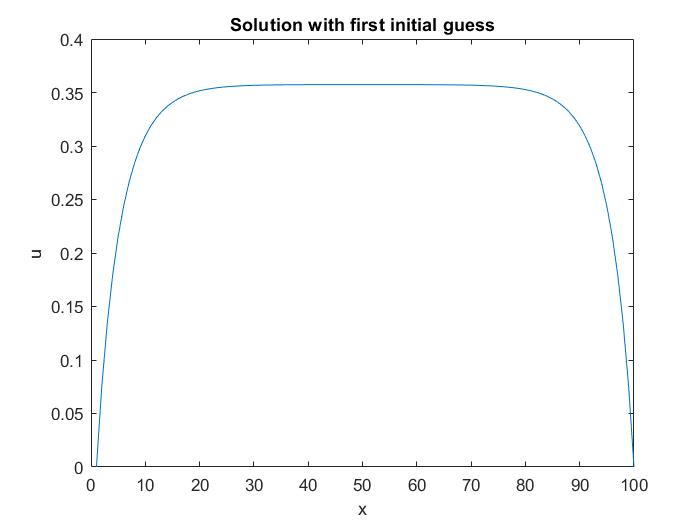
\includegraphics[width=0.32\linewidth]{code/p3_1.jpg}}   
   {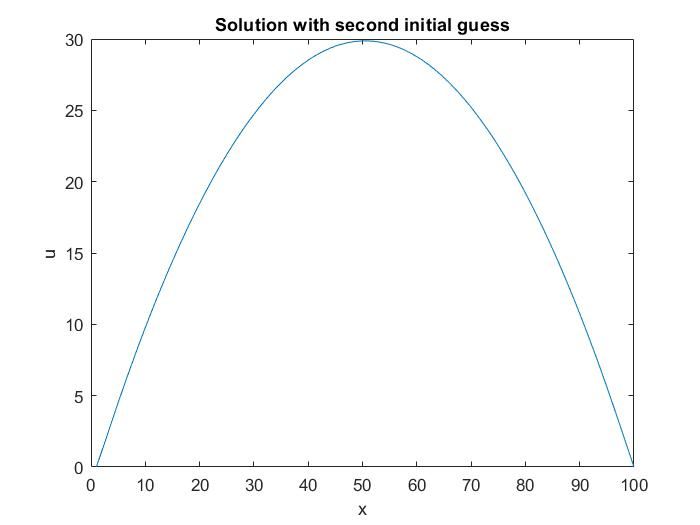
\includegraphics[width=0.32\linewidth]{code/p3_2.jpg}}
   {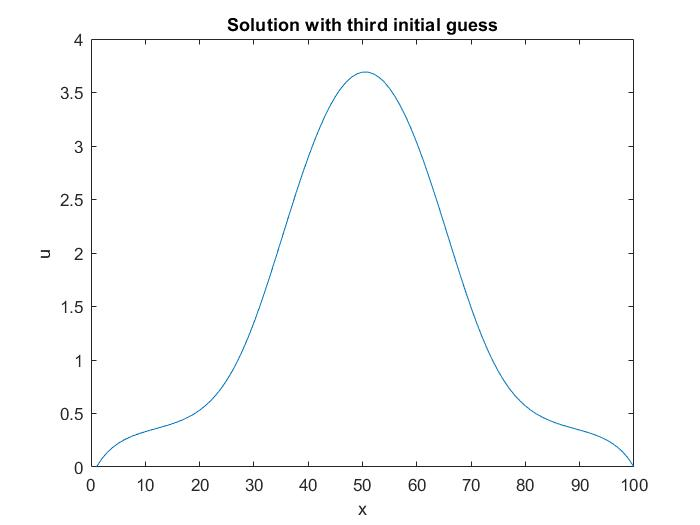
\includegraphics[width=0.32\linewidth]{code/p3_3.jpg}}
  \caption{The stable solutions for the nonlinear PDE defined in Problem No.3 where different initial guesses give different solutions. The nonlinear system of equations was solved using Newton method with Line Search on 100 mesh points.}
   \label{fig:prob3}
\end{figure} 